\begin{frame}
\frametitle{Age Regression}
Linear Gaussian Process Regression to predict subject ages.
\begin{columns}[c]
\column{0.5\textwidth}
\includegraphics[width=1\textwidth]{age_loglikelihood}
\column{0.5\textwidth}
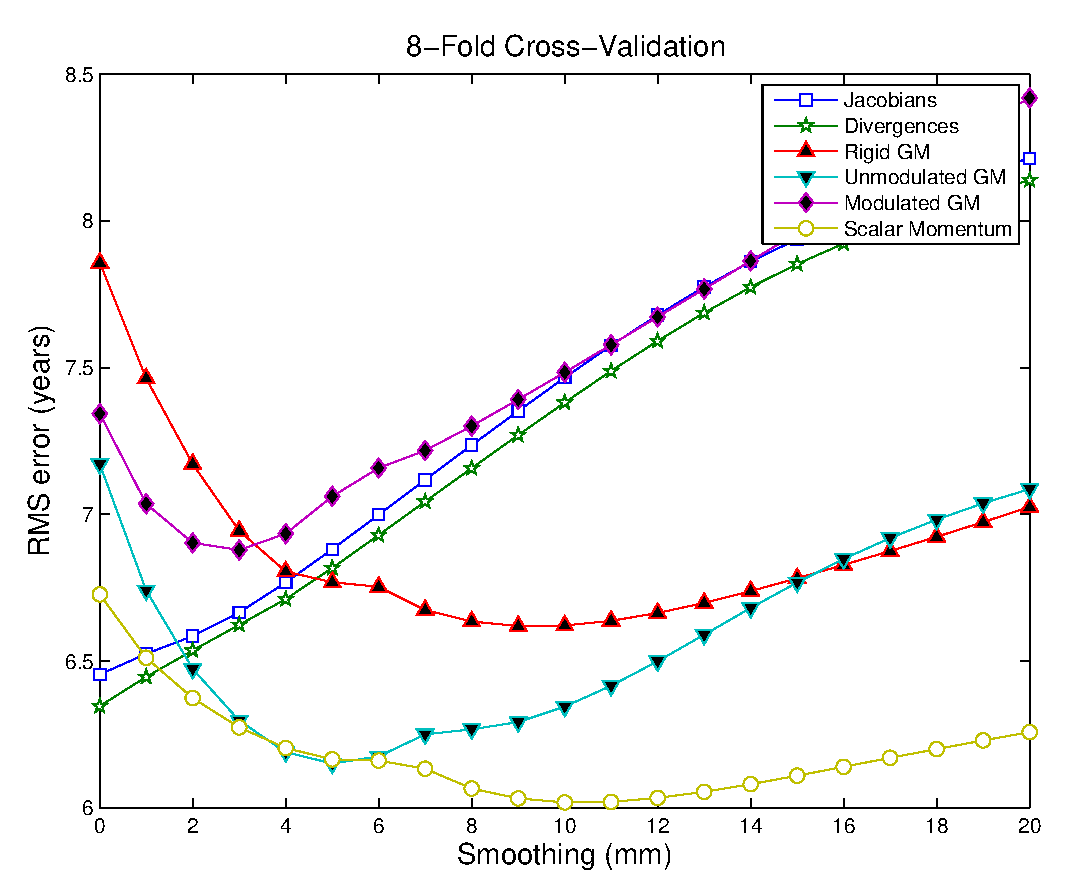
\includegraphics[width=1\textwidth]{age_rms}
\end{columns}

\begin{tiny}
Rasmussen, CE \& Williams, CKI. \emph{Gaussian processes for machine learning}. Springer (2006).

\end{tiny}
\end{frame}

%%%%%%%%%%%%%%%%%%%%%%%%%%%%%%%%%%%%%%%%%%%%%%%%%%%%%%%%%%%%%%%
\begin{frame}
\frametitle{Sex Classification}
Linear Gaussian Process Classification (EP) to predict sexes.
\begin{columns}[c]
\column{0.5\textwidth}
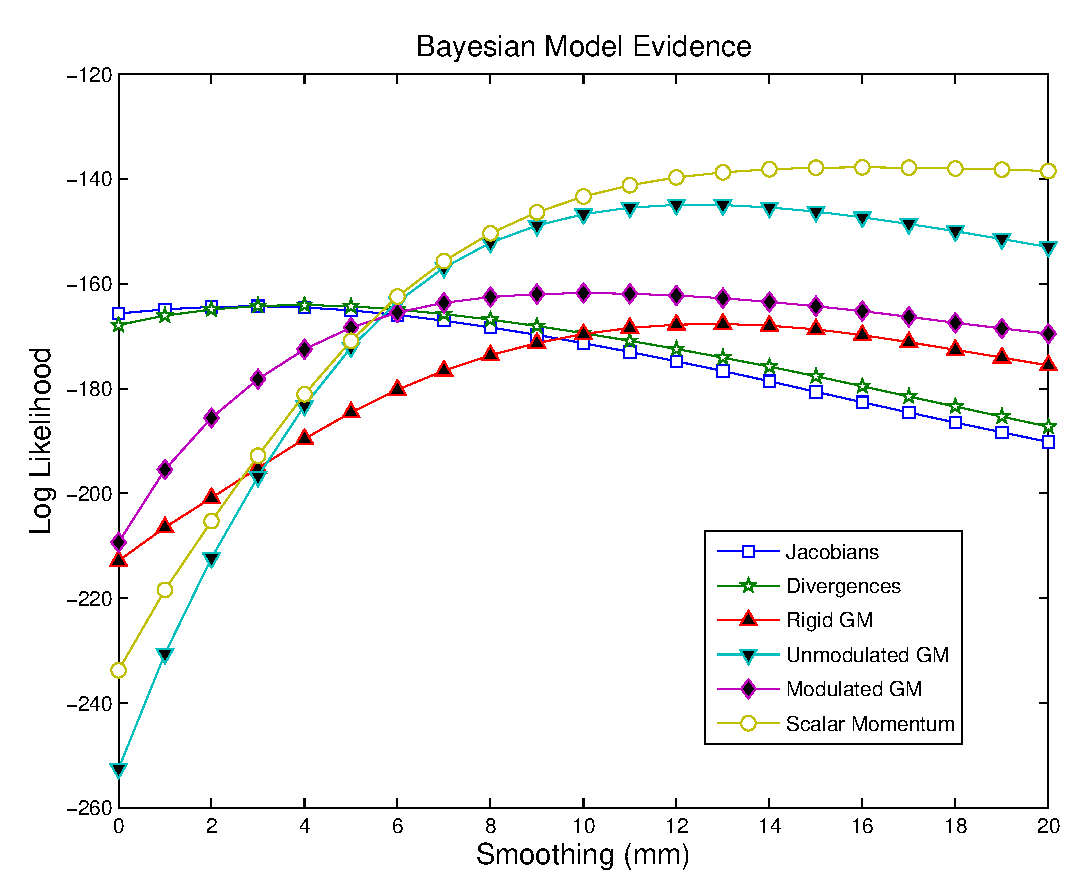
\includegraphics[width=1\textwidth]{sex_loglikelihood}
\column{0.5\textwidth}
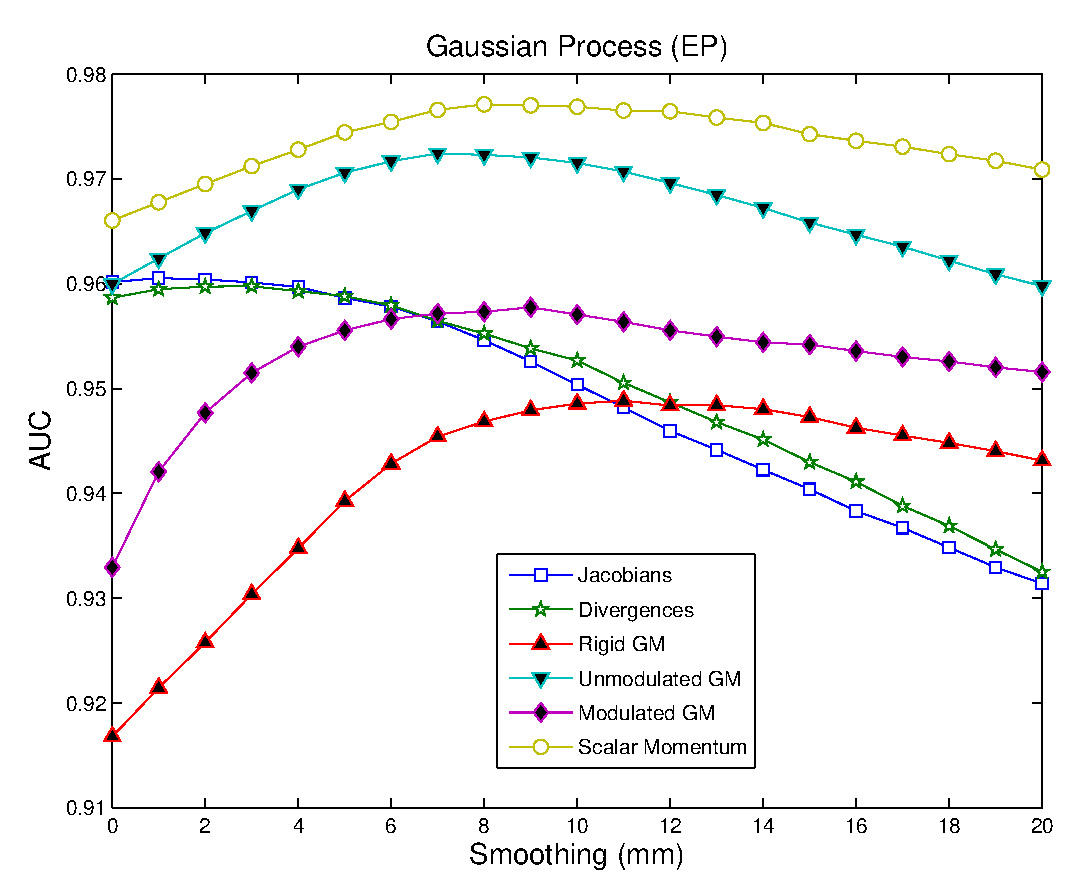
\includegraphics[width=1\textwidth]{sex_auc_GP}
\end{columns}

\begin{tiny}
Rasmussen, CE \& Williams, CKI. \emph{Gaussian processes for machine learning}. Springer (2006).

\end{tiny}
\end{frame}

%%%%%%%%%%%%%%%%%%%%%%%%%%%%%%%%%%%%%%%%%%%%%%%%%%%%%%%%%%%%%%%
%\begin{frame}
%\frametitle{Sex Classification}
%Linear SVM versus Gaussian Process Classification (EP).
%\begin{columns}[c]
%\column{0.5\textwidth}
%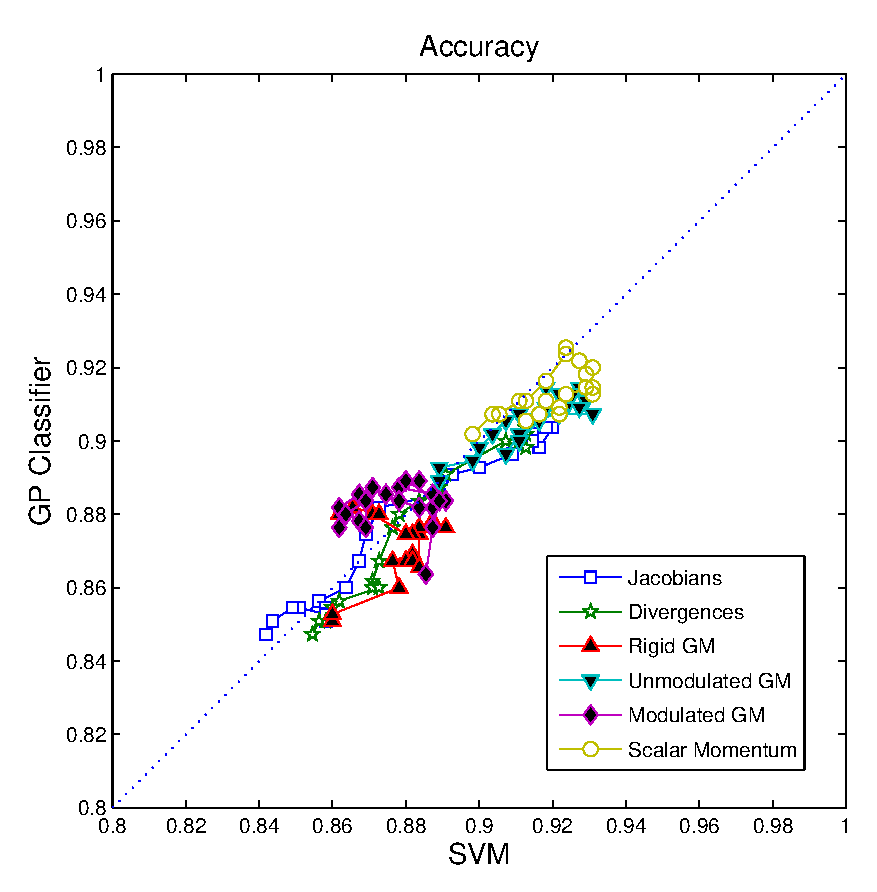
\includegraphics[width=1\textwidth]{sex_SVM_v_GP_acc}
%\column{0.5\textwidth}
%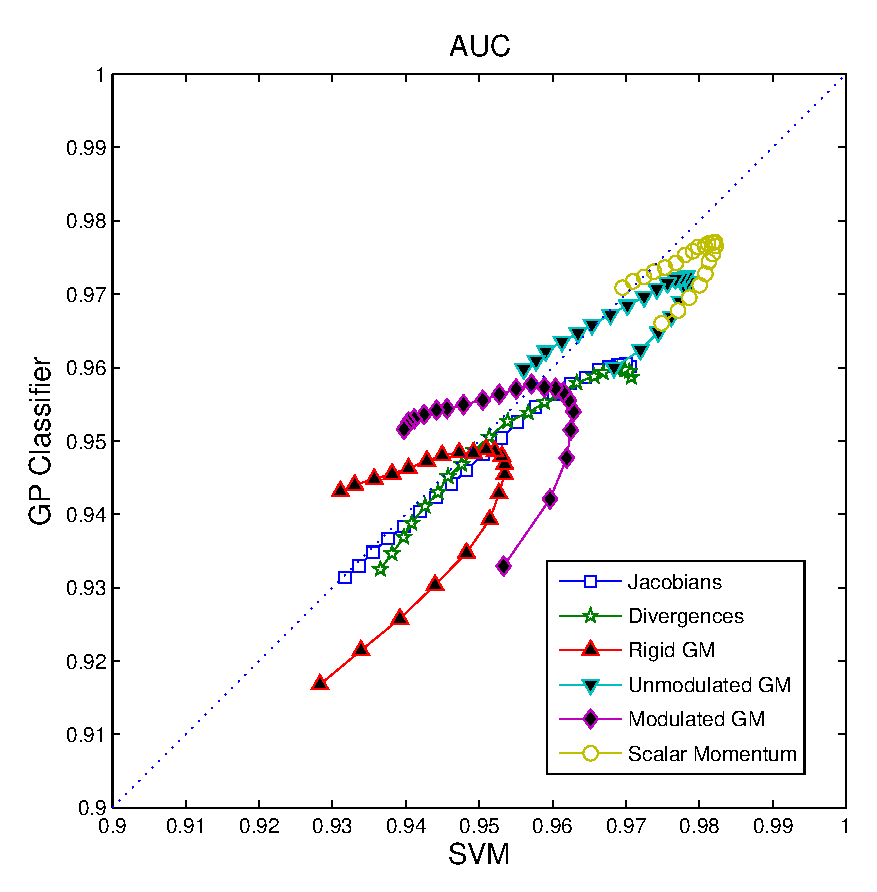
\includegraphics[width=1\textwidth]{sex_SVM_v_GP_AUC}
%\end{columns}
%\end{frame}

%%%%%%%%%%%%%%%%%%%%%%%%%%%%%%%%%%%%%%%%%%%%%%%%%%%%%%%%%%%%%%%

\begin{frame}
\frametitle{Predictive Accuracies}
\begin{columns}[c]
\column{0.5\textwidth}

Age

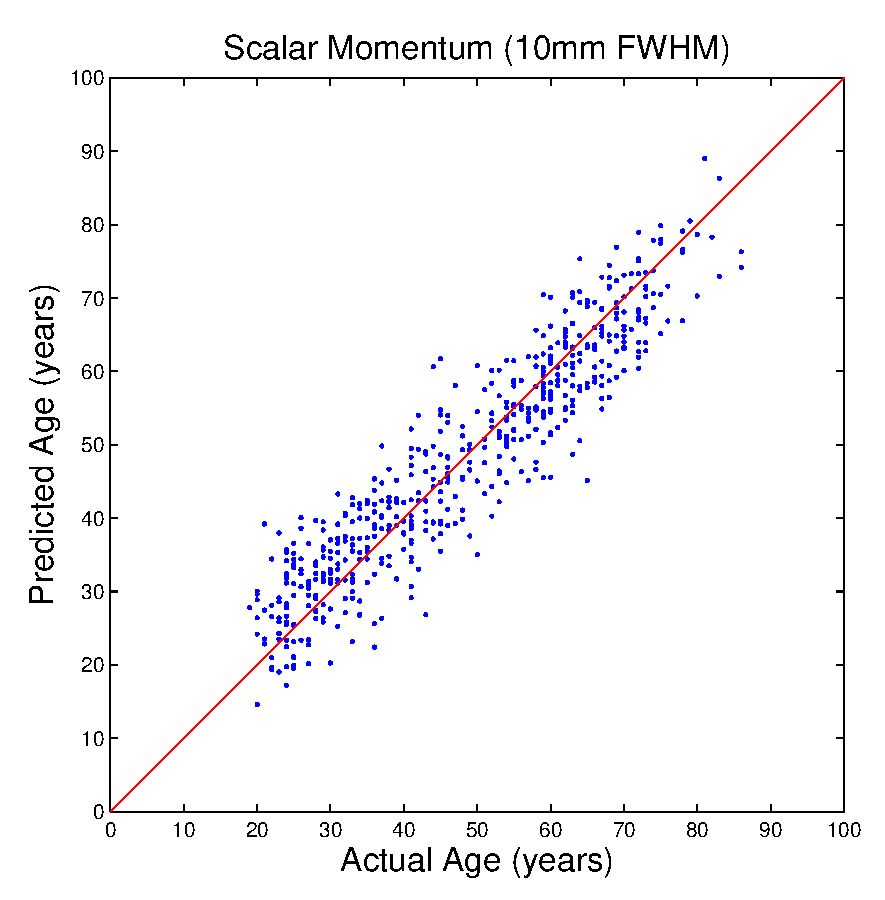
\includegraphics[width=1\textwidth]{age_predictions}
\column{0.5\textwidth}

Sex

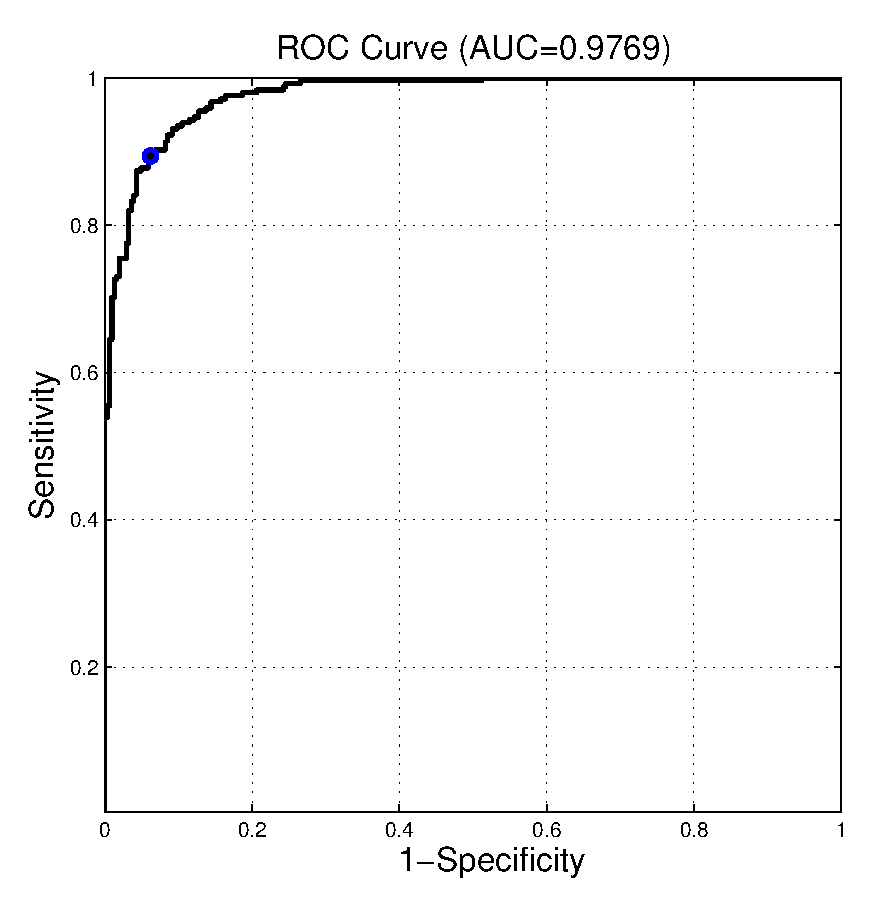
\includegraphics[width=1\textwidth]{sex_roc}
\end{columns}
\end{frame}

\begin{frame}
\frametitle{Conclusions}
\begin{itemize}
\item{Scalar momentum (with about 10mm smoothing) appears to be a useful feature set.}
\item{Jacobian-scaled warped GM is surprisingly poor.}
%\item{SVC slightly more accurate than GP (but we knew that already).}
\item{Amount of spatial smoothing makes a big difference.}
\item{Further dependencies on the details of the registration still need exploring.}
\end{itemize}
\end{frame}
%%%%%%%%%%%%%%%%%%%%%%%%%%%%%%%%%%%%%%%%%%%%%%%%%%%%%%%%%%%%%%%
%\begin{frame}
%\frametitle{Additional references}
%\begin{itemize}
%\item{Ashburner, J \& Kl\"oppel, K. \emph{Multivariate models of inter-subject anatomical variability}. NeuroImage 56(2):422--439 (2011).}
%\item{Ashburner, J \& Friston, KJ. \emph{Diffeomorphic registration using geodesic shooting and Gauss-Newton optimisation}. NeuroImage 55(3):954--967 (2011).}
%\end{itemize}
%\end{frame}

\begin{frame}
\begin{center}
\includegraphics[width=.8\textwidth]{hyper_male}
\end{center}
\end{frame}

\begin{frame}
\begin{center}
\includegraphics[width=.8\textwidth]{avgT1}
\end{center}
\end{frame}

\begin{frame}
\begin{center}
\includegraphics[width=.8\textwidth]{hyper_female}
\end{center}
\end{frame}


